\documentclass[conference]{IEEEtran}
\IEEEoverridecommandlockouts
% The preceding line is only needed to identify funding in the first footnote. If that is unneeded, please comment it out.
\usepackage{cite}
\usepackage{amsmath,amssymb,amsfonts}
\usepackage{algorithmic}
\usepackage{graphicx}
\usepackage{textcomp}
\usepackage{xcolor}
\def\BibTeX{{\rm B\kern-.05em{\sc i\kern-.025em b}\kern-.08em
    T\kern-.1667em\lower.7ex\hbox{E}\kern-.125emX}}
\begin{document}

\title{Visualizing Software Evolution in Linux: A Hierarchical Graph-Based Heat Map Approach\\

\thanks{}
}

\author{\IEEEauthorblockN{Adrian Volpe}
\IEEEauthorblockA{\textit{College of Science and Math} \\
\textit{Belmont University}\\
Nashville, USA \\
adrianvolpemath@gmail.com}
\and
\IEEEauthorblockN{Esteban Parra}
\IEEEauthorblockA{\textit{College of Science and Math} \\
\textit{Belmont University}\\
Nashville, USA \\
esteban.parrarodriguez@belmont.edu}}

% Try using this alternative long format instead if modifying the original leads to it looking weird
% \author{\IEEEauthorblockN{Michael Shell\IEEEauthorre
% fmark{1}, Homer Simpson\IEEEauthorrefmark{2}, James K
% irk\IEEEauthorrefmark{3}, Montgomery Scott\IEEEautho
% rrefmark{3} and Eldon Tyrell\IEEEauthorrefmark{4}}
% \IEEEauthorblockA{\IEEEauthorrefmark{1}School of Ele
% ctrical and Computer Engineering\\
% Georgia Institute of Technology, Atlanta, Georgia 30
% 332--0250\\
% Email: mshell@ece.gatech.edu}
% \IEEEauthorblockA{\IEEEauthorrefmark{2}Twentieth Cen
% tury Fox, Springfield, USA\\
% Email: homer@thesimpsons.com}


\maketitle

\begin{abstract}
This project presents a visualization of Linux commit activity using a hierarchical, heat-map based graph. Using a large dataset of commit data from Zenodo, we model the Linux structure as a directed hierarchy. Each node in the graph represents a subsystem, and edges show a parent-child relationship within the Linux architecture. The graph is rendered radially in Unity with a color gradient applied to nodes to indicate the volume of commits made to each subsystem. The result is an interactive, intuitive view of development hotspots in the Linux kernel, aimed at supporting further software evolution analysis. 
\end{abstract}

\begin{IEEEkeywords}
commit, graph, heat-map
\end{IEEEkeywords}

\section{Introduction}
Linux is a family of open source operating systems that are based on the Linux kernel. The Linux kernel is a core component of a device that manages the hardware and resources. It's responsible for the CPU, memory and peripherals. Linux is versatile and is used everywhere from powering smartphones to operating smart TV's. Linux is fast, secure and highly scaleable, so it is important to learn how Linux changes over time.% talk about what a linux is and what it does and why its useful (free, safe, fast)

Linux is an open source system, meaning that the source code is available, for free, to be modified and redistributed. However, the main Linux operating system (OS) is only modified by specific authors and each modification is checked thoroughly. These changes to the Linux OS source code are called commits. Each commit contains certain data including: the author of the commit, the time the commit was made, every line changed, and the number of added and deleted lines. Commits are used to keep track of what code was changed, when it was changed and by who. % what is linux/ what is linux used for / what are commits / what are commits used for /  


%maybe talk about heirarchical ghraphs in here and why they are useful for visualization rthings

Analyzing commit history is useful because it can show areas in the Linux kernel that have not recently been modified or that have been modified heavily. Areas that have recently been modified often are more likely to contain bugs or errors. Thus commit history visualization can strengthen our ability to find bugs in the Linux OS. We created a graph visualization of Linux subsystems using commit frequency as a heat metric. This visualization is specifically useful because it provides an interactive and clear way of seeing commit history. This approach has not been done before and can provide a new way of seeing the relationship between the Linux OS structure and how commits are distributed across it. % why is this useful/ why is looking at commit activity useful / how is this different

We will discuss some related works, the methods used to create this graph, results, and areas of future improvement.




\section{Related Work}

% read papers, summarize each one individually, then look at every summary and answer these questions in the paper: what is known? what is unknown? what has been done? what are you doing? how are they different? or do it this way : GENERAL OVERVIEW WHAT BEEN DONE, go through each paper and explain, GENERAL OVERVIEW WHA+Y DIFFERENT.

I have added something to the LaTeX file, now will it show up on GitHub? Im gonna add even more chnages like this one here. Let me make a change here and see where it appears when I hit save.

\section{Methodology}

\subsection{Data Collection}
The data we used came from the Zenodo dataset provided by VISSOFT. This data was given to us in the form of a JavaScript Object Notation (JSON) file. To read this file we created a program in Java to parse through the data and output a text file. The program first looked at each subsystem and the parent-child relationships between them, then how many commits were made to that subsystem. This text file is what we use to construct and render the graph.

\subsection{Color Encoding}
At first, almost all nodes took on a nearly indistinguishable shade of green, except for a select few nodes. This was because the range of commits made to subsystems was huge. The maximum number of commits made to a subsystem was 500,000 while the minimum was 0. The average was somewhere around 1000 commits per subsystem. Thus, when we colored each node by taking a ratio between each subsystems number of commits by the maximum number of commits it heavily skewed the nodes to be green. To fix this we implemented a logarithmic scale. The color of each node is now determined by the log of that previous ratio, except in cases where the ratio becomes $0$ or $1$. Those cases are handled individually, since $\log(0)$ is undefined and $\log(1)$ returns a green color which is the opposite of what is desired when the ratio is $1$. This logarithmic scaling fixed the issue with most nodes looking identical. Nodes now take on a range of colors from green to red.

\subsection{Graph Construction}
To construct the graph we created C\# code in Unity to read the text file output from Java. The text file contained the parent-child relationships between all of the subsystems, the exact number of commits made to each subsystem, and a color corresponding to each node. Our code created a set of nodes and a set of vertices based on this text file. A node is created to represent each subsystem and its corresponding color, and an edge connects two nodes if and only if one is a child of the other. This creates a hierarchical graph layout that not only shows us the relationships between the subsystems, but also the relative commit frequency between them as well. This graph is then visualized using a radial layout so that the nodes are spaced evenly along different radii.

\subsection{Implementation}
The implementation of this graph in Unity is interactive. The user is able to zoom in/out and pan the camera. The user is also able to click on each node to view information about that subsystem. On click the user can see the name of the subsystem and the exact number of commits made to that subsystem. 

\begin{figure}[h!]
	\centering
	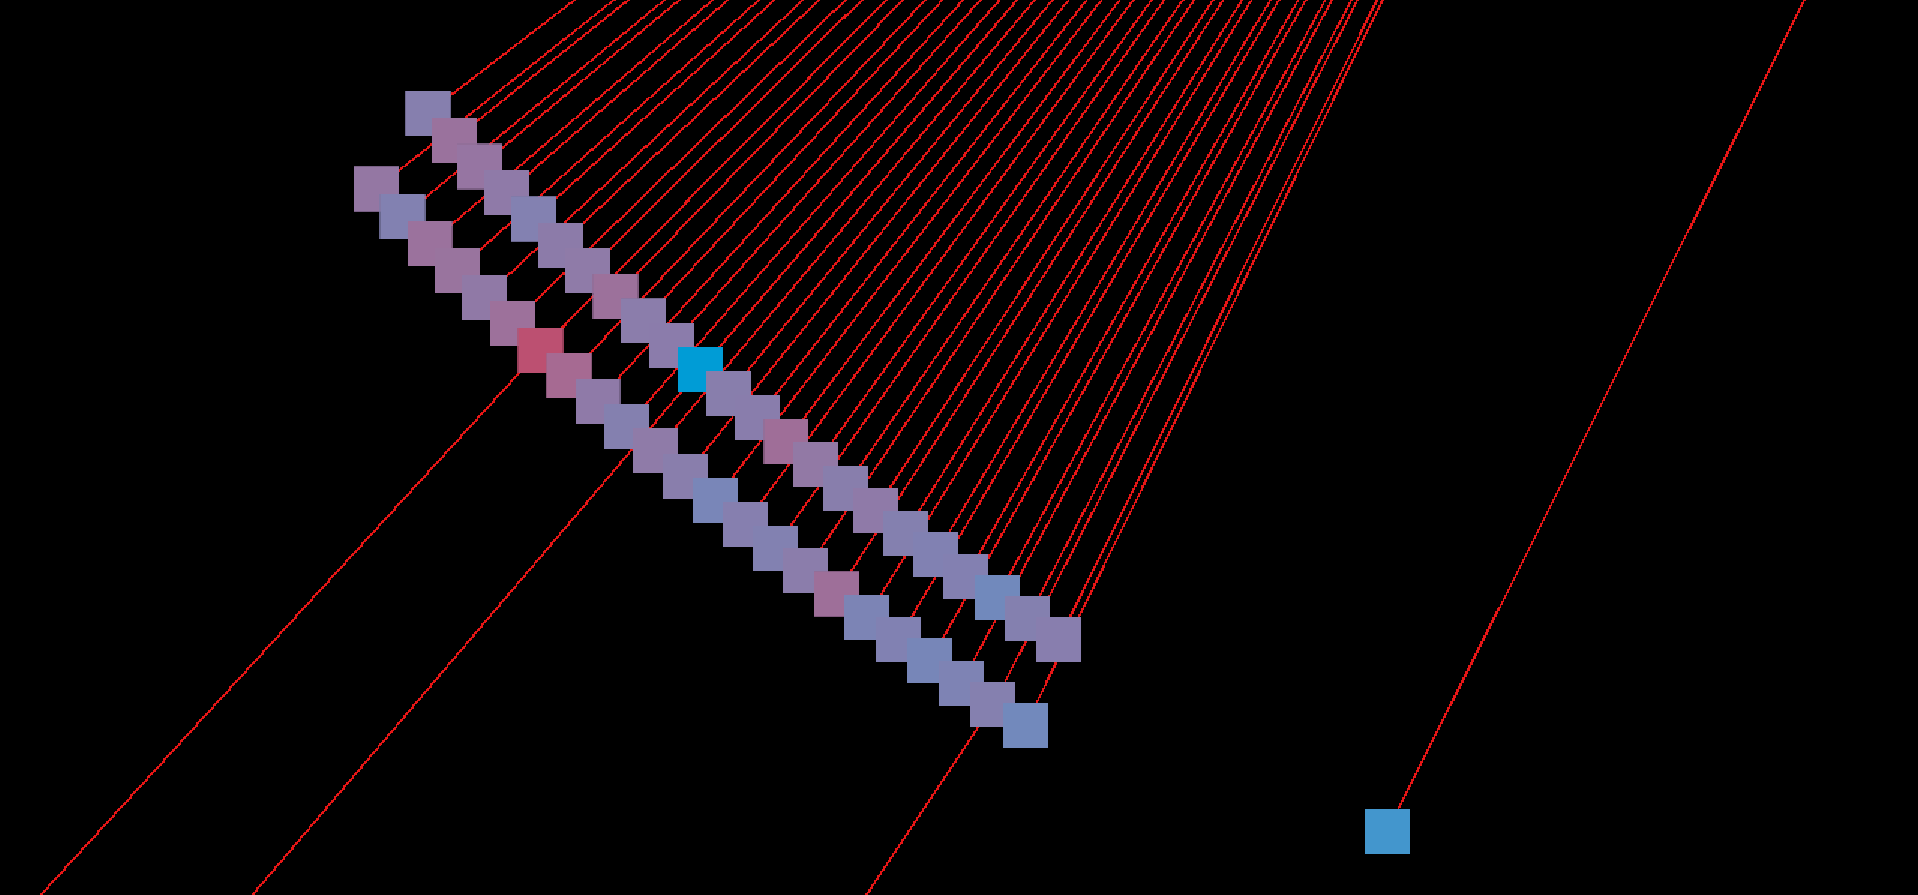
\includegraphics[width=0.45\textwidth]{randomSection.png}
	\caption{This image shows a variety of colors attributed to nodes based on commit frequency of that subsystem.}
\end{figure}

\section{Results}

talk about scalability issues, groups of high commit frequency, and think of other things to talk about as well.

\section{Discussion}

talk about future directions except you plan on doing some of those future directions so i don teven know what man. talk about using git clone instead of java text file reading output roundabout stupid way.

\section{Conclusion}


\section{References}



\begin{thebibliography}{00}
\bibitem{b1} G. Eason, B. Noble, and I. N. Sneddon, ``On certain integrals of Lipschitz-Hankel type involving products of Bessel functions,'' Phil. Trans. Roy. Soc. London, vol. A247, pp. 529--551, April 1955.
\bibitem{b2} J. Clerk Maxwell, A Treatise on Electricity and Magnetism, 3rd ed., vol. 2. Oxford: Clarendon, 1892, pp.68--73.
\bibitem{b3} I. S. Jacobs and C. P. Bean, ``Fine particles, thin films and exchange anisotropy,'' in Magnetism, vol. III, G. T. Rado and H. Suhl, Eds. New York: Academic, 1963, pp. 271--350.
\bibitem{b4} K. Elissa, ``Title of paper if known,'' unpublished.
\bibitem{b5} R. Nicole, ``Title of paper with only first word capitalized,'' J. Name Stand. Abbrev., in press.
\bibitem{b6} Y. Yorozu, M. Hirano, K. Oka, and Y. Tagawa, ``Electron spectroscopy studies on magneto-optical media and plastic substrate interface,'' IEEE Transl. J. Magn. Japan, vol. 2, pp. 740--741, August 1987 [Digests 9th Annual Conf. Magnetics Japan, p. 301, 1982].
\bibitem{b7} M. Young, The Technical Writer's Handbook. Mill Valley, CA: University Science, 1989.
\end{thebibliography}
\vspace{12pt}


\end{document}